\documentclass[10pt,a4paper]{article}

\usepackage[utf8]{inputenc}
\usepackage[spanish]{babel}
\usepackage{graphicx}
\usepackage{fancyhdr}
\usepackage[skip=6pt]{caption}
\usepackage{multicol}
%\usepackage[hidelinks]{hyperref}

\title{Interpretación remota de partituras sobre instrumentos de viento}
\author{Víctor Manuel Fernández Castro}
\date{Abril de 2016}

\setlength{\parskip}{6pt}
\fancyhead[L]{Víctor M. Fdez. Castro}
\renewcommand{\footrulewidth}{0.4pt}
\setlength{\headheight}{13.07225pt} 

% ------------------------------------------------------------------------------

\begin{document}
	
	% Portada ------------------------------------------------------------------
	
	\maketitle
	\thispagestyle{empty}
	
	% Índice -------------------------------------------------------------------
	
	\newpage
	\tableofcontents
	\listoffigures
	
	% Capítulo 1 ---------------------------------------------------------------
	
	\newpage
	\pagestyle{fancy}
	\section{Introducción y objetivos}
	
	Nuestro proyecto parte de la atención en numerosas iglesias de Granada, que
	incorporan órganos de tubos, instrumentos muy complejos, muchos de ellos
	formando parte del inmobiliario, y merecedores de un gran reconocimiento por
	la artesanía y la calidad de su construcción.
	
	Lamentablemente, muchos de ellos se encuentran en un estado de abandono, lo
	que acelera su deterioro, no se reparan y, por ello, no se pueden tocar,
	cayendo en un círculo vicioso.
	
	Además, creemos interesante la idea de que se pueda hacer sonar un órgano
	aunque no haya organista, dando la posibilidad tanto de acompañar
	celebraciones litúrgicas como de tener música de fondo durante el horario de
	visitas.
	
	\subsection{Objetivos}
	
	Nuestro propósito es ingeniar un sistema capaz de \textbf{interpretar
	partituras musicales en un órgano} suplantando las pulsaciones del artista,
	lo que incluye los siguientes objetivos:
	
	\begin{enumerate}
		\item Analizar la \textbf{mecánica real} de un órgano eclesiástico.
		
		\begin{enumerate}
			\item Tomar \textbf{medidas completas} de cada uno de los teclados,
			los pedales y las palancas de registros.
			\item \textbf{Diseñar en 3D} los componentes principales del
			instrumento.
			\item Determinar la \textbf{presión} necesaria para mover cada
			tecla, cada pedal y cada palanca del órgano.
		\end{enumerate}
		
		\item Estudiar la comunicación entre el \textit{software} y el
		\textit{hardware}, incluyendo todos los \textbf{componentes
		electrónicos} que habrá de incluir.
		
		\item Plantear distintas \textbf{alternativas de sistemas empotrados}
		que sirvan de soporte de programación.
		
		\item Analizar el \textbf{protocolo MIDI} como formato de archivo para
		almacenar partituras.
		
		\item \textbf{Diseñar} el sistema \textit{software} que cubrirá varias
		vías de comunicación entre el usuario y la mecánica, lo que comprende:
		
		\begin{enumerate}
			\item Un \textbf{servicio en segundo plano}, que atienda:
			
			\begin{enumerate}
				\item Reproducción de archivos MIDI.
				\item Comunicación inter-proceso.
				\item Receptor de un mando a distancia.
				\item Menú de control sobre el hardware, con un ''modo
				Ingeniería''.
			\end{enumerate}
			
			\item Una \textbf{aplicación \textit{web}} para controlar el
			sistema, con soporte para:
			
			\begin{enumerate}
				\item Reproducir partituras electrónicas.
				\item Instalar nuevas piezas y gestionar listas de reproducción.
				\item Configurar el mando a distancia.
			\end{enumerate}
			
			\item Una \textbf{base de datos} como soporte de almacenamiento
			persistente.
			\item Un \textbf{protocolo de comunicación} entre la aplicación
			y el servicio.
		\end{enumerate}
		
		\item \textbf{Implementar} el sistema diseñado, como:
		
		\begin{enumerate}
			\item Un demonio para Linux.
			\item Un servicio \textit{web} sobre Apache y PHP.
			\item Una base de datos MySQL.
		\end{enumerate}
		
		\item \textbf{Validar} junto al \textit{hardware} el proyecto
		desarrollado.
	\end{enumerate}
	
	El diseño del sistema electrónico, que requiere competencias de Ingeniería
	Electrónica e Industrial, fue objeto del proyecto de D. Mikel Aguayo
	Fernández.
	
	% Capítulo 2 ---------------------------------------------------------------
	
	\section{Requisitos técnicos}
	
	Para especificar el diseño de este proyecto hemos propuesto una serie de
	requisitos tanto \textit{hardware} como \textit{software}, que enumeramos a
	continuación.
	
	\subsection{Requisitos hardware}
	
	\begin{enumerate}
	
		\item Un juego de mecanismos accionará las \textbf{teclas}, otro moverá
		los \textbf{pedales} y otro desplazará los \textbf{registros} de
		timbres.
		
		\item El sistema no podrá acceder a la mecánica interna del instrumento,
		ni modificarlo de ninguna forma.
		
		\item No podrá apoyarse demasiado peso sobre el órgano, ni hacerse
		contra-apoyo (hacia arriba).
		
		\item El \textbf{control principal}, la instalación de partituras y la
		configuración se harán \textbf{remotamente}.
		
		\item Se proveerá un \textbf{control local reducido} de los accionadores
		con fines de puesta en marcha y mantenimiento.
		
		\item Asimismo se facilitará el control remoto desde un \textbf{mando a
		distancia}.
		
		\item El diseño debe ser \textbf{flexible y extensible} para distintos
		órganos.
		
		\item Se debe de poder instalar y desinstalar fácilmente.
		
	\end{enumerate}
	
	\subsection{Requisitos software}
	
	\begin{enumerate}
		
		\item Se ofrecerá \textbf{control remoto} para todos los casos de uso a
		nivel de usuario.
		
		\item La interfaz permitirá controlar la \textbf{reproducción}: iniciar
		una pieza, pausarla, reanudarla y detenerla. La reproducción por defecto
		será en modo bucle.
		
		\item Facilitará la subida y \textbf{gestión de partituras}. En dicho
		gestor se mostrará la duración de cada pieza.
		
		\item Los archivos a procesar son de formato \textbf{MIDI estándar}, sin
		perjuicio de que una partitura pueda estar adaptada específicamente al
		sistema.
		
		\item Las piezas musicales se clasificarán en \textbf{listas de
		reproducción}.
		
		\item La interfaz de usuario permitirá \textbf{asignar} dichas listas a
		ciertos botones del mando arriba mencionado.
		
		\item El \textbf{mando} tendrá capacidad para reproducir una serie de
		listas programadas, así como pausar y detener la reproducción.
		
		\item El \textit{software} dará soporte al \textbf{testeo} de los
		accionadores de forma local.
		
		\item El controlador debe ser \textbf{extensible} para órganos con más o
		menos teclas, distinto número de teclados o diferente configuración de
		registros.
		
		\item La aplicación para el usuario debe ser lo más \textbf{sencilla e
		intuitiva} posible.
		
		\item Se busca obtener una aplicación de control
		\textbf{multiplataforma}.
		
		\item La interfaz de usuario se presentará en varios \textbf{idiomas}.
		
		\item Ya que el control es remoto, se hará hincapié en la
		\textbf{seguridad}, tanto autentificación de acceso como aspectos de
		programación, tales como inyección de código.
		
	\end{enumerate}
	
	% Capítulo 3 ---------------------------------------------------------------
	
	\section{Análisis del sistema}

	Como paso previo al diseño del sistema, deberemos conocer con detalle todos
	los elementos con los que va a interactuar nuestro sistema, así como
	plantear diferentes alternativas de cara al desarrollo del
	\textit{software}.

	\subsection{Órgano de la Parroquia de Santa Fe}

	El instrumento instalado en la Parroquia de la Encarnación de Santa Fe es en
	realidad un doble órgano artesanal construido en dos fases: En 1775 se
	instaló el primer órgano, de estilo \textbf{barroco}, obra del organero
	Pedro Ghys. Posteriormente, a principios de la década de 1830, el francés
	Guillermo D'Enoyer lo amplía añadiendo un órgano \textbf{romántico}, con un
	segundo teclado y nuevos sonidos, pero todo el mecanismo es independiente
	del primer instrumento.
	

	\begin{multicols}{2}
		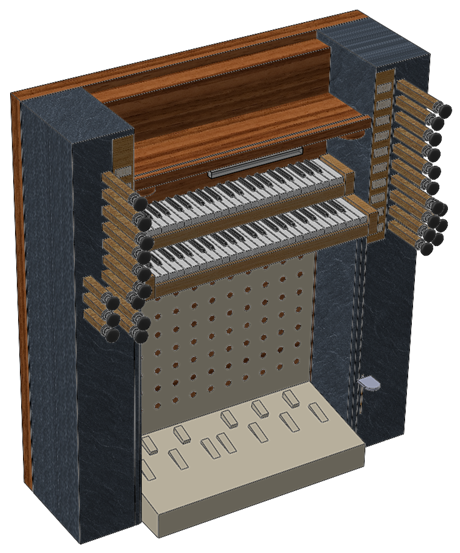
\includegraphics[width=0.4\textwidth]{images/organo}
		
		La primera tarea que llevamos a cabo fue 
		conocer el órgano en profundidad, tomar 
		algunas medidas y \textbf{diseñar el modelo en 3D} 
		con el \textit{software} \textit{SolidWorks}.
	\end{multicols}
	
	\subsection{PCB de control}
	
	\subsection{SBC Raspberry pi}
	
	\subsection{Formato de archivo MIDI}
	
	% Capítulo 4 ---------------------------------------------------------------
	
	\section{Diseño e implementación}
	
	\subsection{Planteamiento}
	
	\subsection{Servicio del reproductor}
	
	\subsection{Interfaz web}
	
	\subsection{Base de datos}
	
	\subsection{Aplicaciones auxiliares}
	
	\subsection{Resultado}
	
	% Capítulo 5 ---------------------------------------------------------------
	
	\section{Validación y verificación}
	
	% Capítulo 6 ---------------------------------------------------------------
	
	\section{Conclusión}

\end{document}
